\documentclass[11pt,letterpaper]{article}
\usepackage[utf8]{inputenc}
\usepackage[T1]{fontenc}
\usepackage[spanish,es-nodecimaldot]{babel}
\usepackage{lmodern,microtype}
\usepackage[margin=2.25cm]{geometry}
\usepackage{xcolor,graphicx,booktabs,tabularx,array,longtable,float,xurl,hyperref,fancyhdr}
\usepackage{tikz}
\usetikzlibrary{arrows.meta,positioning,shapes.geometric}
\definecolor{AtoyacBlue}{HTML}{244E60}
\definecolor{AtoyacGreen}{HTML}{52785D}
\definecolor{AtoyacGold}{HTML}{B58A3A}
\hypersetup{colorlinks=true,linkcolor=AtoyacBlue,urlcolor=AtoyacBlue}
\setlength{\parindent}{0pt}
\setlength{\parskip}{5pt}
\pagestyle{fancy}\fancyhf{}
\setlength{\headheight}{14pt}
\lhead{Proyecto Alto Atoyac}\rhead{Reporte sintético}\cfoot{\thepage}
\newcommand{\limite}[1]{\begin{center}\fcolorbox{AtoyacGold}{yellow!8}{\parbox{.91\textwidth}{\textbf{Límite de interpretación.} #1}}\end{center}}
\newcommand{\idea}[1]{\begin{center}\fcolorbox{AtoyacGreen}{green!4}{\parbox{.91\textwidth}{#1}}\end{center}}

\title{\textbf{Análisis geo-estadístico para tratamiento de aguas residuales en la cuenca del Alto Atoyac:}\\[6pt]\Large Concentraciones territoriales de actividades textiles\\[4pt]\large Síntesis para discusión y toma de decisiones}
\author{\textbf{Universidad de las Américas Puebla}\\[12pt]Nuria Arroyo Bustamante\\173605}
\date{24 de septiembre de 2026}

\begin{document}
\maketitle
\thispagestyle{empty}
\vfill
\idea{Este documento explica dónde se concentran las unidades económicas textiles y qué preguntas conviene investigar en cada territorio. No identifica responsables de contaminación ni propone trazos de colectores.}
\vfill
\begin{center}\small Documento sintético. Los resultados, métodos, tablas auditables y rutas de archivos se documentan en el reporte maestro.\end{center}
\newpage
\tableofcontents
\newpage

\section{Resumen ejecutivo}

El estudio respondió una pregunta previa a cualquier decisión de infraestructura: \textbf{¿en qué zonas de la cuenca del Alto Atoyac se concentran las unidades económicas textiles, de confección y de lavandería/tintorería, y qué perfil productivo tiene cada concentración?} La información disponible permitía ubicar establecimientos individuales, pero no ofrecía una lectura regional comparable ni separaba con claridad actividad sectorial, indicios de uso de agua y evidencia verificada en campo.

Se construyó un universo sectorial auditable de 4,365 establecimientos en 26 municipios. El análisis espacial se hizo con ese universo ampliado para evitar cortes artificiales en el borde de la cuenca; la interpretación se restringió a 4,010 establecimientos dentro de ella. La solución operativa seleccionada reconoce 22 agrupamientos en el universo de detección, de los cuales 18 intersectan la cuenca, y conserva 584 unidades como actividad espacialmente dispersa. Dentro de la cuenca, 578 unidades aparecen como ruido o dispersión.

Los resultados cambian una lectura uniforme del problema. Santa Ana Xalmimilulco destaca por confección, maquila y mezclilla; San Rafael Ixtapalucan y San Miguel Tianguistenco por tejido e hilado; Huejotzingo y el corredor de San Martín Texmelucan combinan manufactura y señales potencialmente húmedas; San Miguel Xoxtla--Coronango y Amozoc forman concentraciones diferenciadas; y Puebla--Cholula--Cuautlancingo aparece como un sistema metropolitano extenso y heterogéneo que requiere subdividir la validación, no tratarse como una sola zona operativa.

La solución seleccionada fue la mejor puntuada bajo una regla documentada, pero dos configuraciones HDBSCAN obtuvieron puntajes prácticamente iguales. La mayor parte de las membresías es estable, aunque existen puntos sensibles y bordes que deben conservarse como incertidumbre. La utilidad del resultado es \textbf{priorizar territorios, recorridos y preguntas}, no inferir descargas ni diseñar infraestructura.

\limite{Concentración espacial $\neq$ contaminación; proximidad a río $\neq$ descarga; cluster $\neq$ zona de servicio; lavandería sectorial $\neq$ lavandería industrial verificada; priorización territorial $\neq$ recomendación de colector.}

\section{Antecedentes y pregunta del estudio}

La cuenca del Alto Atoyac combina urbanización, actividad industrial, manufactura dispersa y una historia documentada de presión sobre el agua. En este contexto, la industria textil y de mezclilla importa porque puede incluir operaciones con necesidades y residuos muy distintos: confección y costura, tejido e hilado, acabado, teñido, lavado, deslavado, limpieza de equipo o servicios de lavandería. El directorio económico no registra de manera completa cuáles de esas operaciones ocurren realmente en cada domicilio ni cuánto agua utilizan.

El problema operativo era doble. Primero, el territorio era demasiado amplio para visitar todas las unidades con la misma intensidad. Segundo, seleccionar únicamente negocios cuyo nombre menciona agua, lavado o teñido podía excluir talleres industriales reales con nombres poco informativos, mientras incluir toda lavandería podía mezclar servicios comerciales con operaciones industriales. El proyecto debía conservar esa incertidumbre y aun así producir una base útil para decidir dónde investigar primero.

La pregunta se formuló en términos territoriales y no acusatorios: localizar concentraciones reproducibles, describir su composición y reconocer qué resultados sobreviven a cambios razonables de parámetros. El análisis no utilizó atributos productivos para formar los clusters; primero se agrupó por proximidad espacial y después se estudió qué actividades estaban presentes en cada grupo. Así se evitó construir de antemano los perfiles que luego se pretendía descubrir.

\section{Construcción del universo}

El punto de partida fue una descarga estatal del Directorio Estadístico Nacional de Unidades Económicas (DENUE) acotada a actividades SCIAN de interés. Tras normalización, control de identificadores y delimitación municipal, se construyó un universo sectorial de 4,365 establecimientos. De ellos, 4,010 se encuentran dentro del polígono de la cuenca. Los 355 puntos exteriores cercanos se conservaron durante la detección para que el límite cartográfico no cortara vecindades reales; después quedaron fuera de la interpretación sustantiva.

El universo sectorial es deliberadamente más amplio que el universo hídrico estricto. Incluye manufactura textil, confección y servicios de lavandería/tintorería potencialmente relevantes. En paralelo se generaron modalidades amplia y estricta, con y sin la fuente MH de trabajo de campo. La regla amplia protege cobertura; la estricta exige señales más directas y excluye lavanderías sin contexto adicional. Ninguna modalidad reemplaza a la otra: muestran el costo de priorizar sensibilidad o especificidad.

MH se conserva como fuente independiente de DENUE porque procede del trabajo de campo de Mary Helen Figueroa y Mayra Jaqueline Ramírez. Cuando fue posible, sus hallazgos se asociaron con identificadores DENUE, sin perder la procedencia. Este vínculo permite auditar coincidencias y diferencias sin presentar la evidencia de campo como si fuera un atributo original del directorio.

\begin{figure}[H]\centering
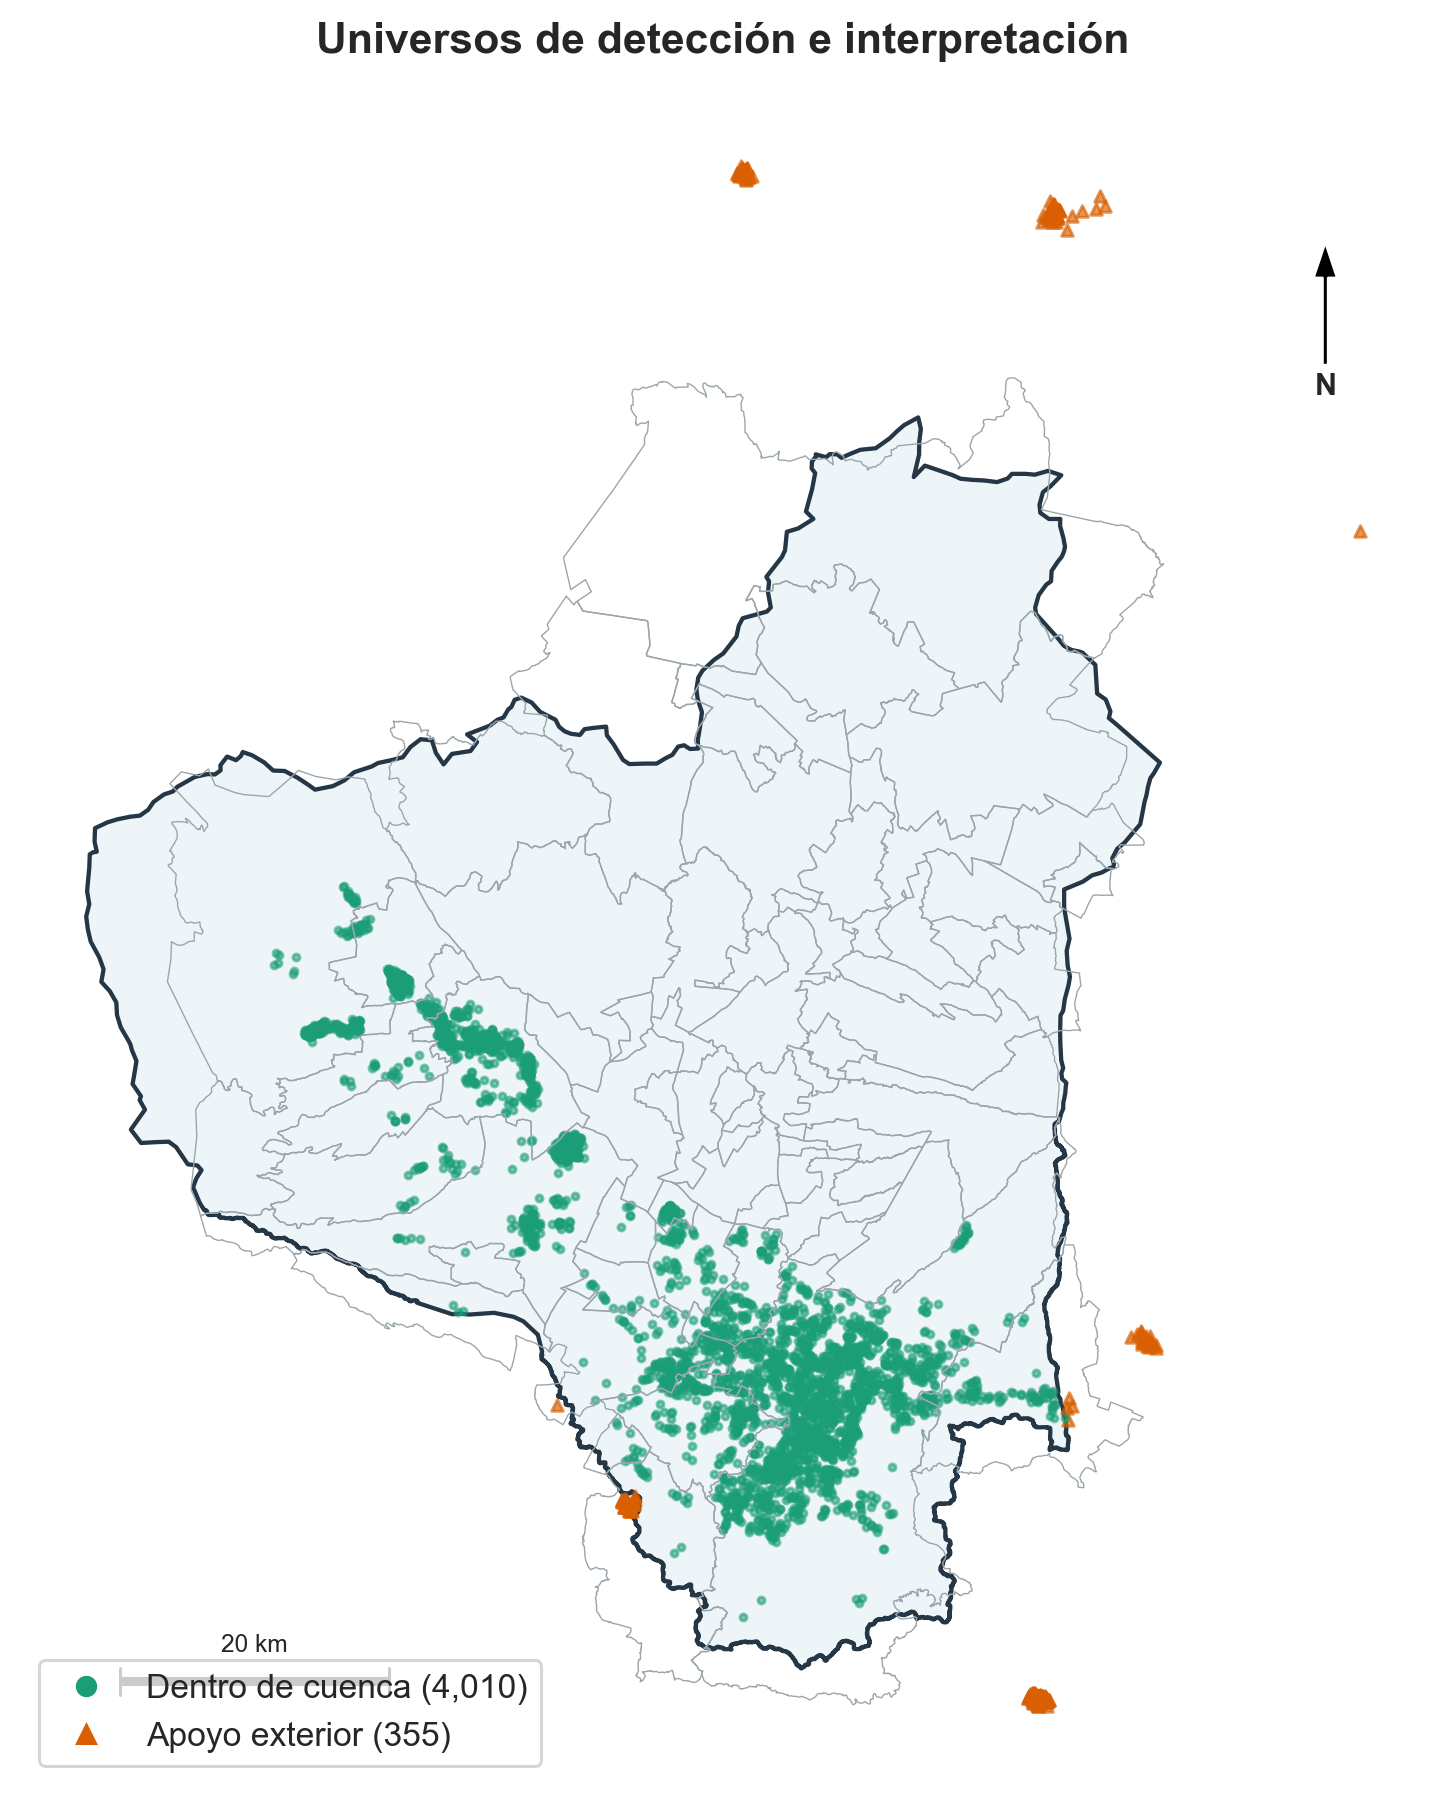
\includegraphics[width=.95\textwidth]{../../outputs/parte_2/13_figuras_finales/01_universos_borde.png}
\caption{Universo ampliado para detección y universo interior para interpretación. Los puntos exteriores controlan el efecto de borde.}
\end{figure}

\limite{DENUE describe ubicación y actividad declarada. No prueba operación actual, proceso húmedo, consumo de agua, descarga, contaminante ni incumplimiento.}

\section{Cómo se detectaron las concentraciones}

Los establecimientos se proyectaron a un sistema métrico y se compararon 57 configuraciones de tres métodos de agrupamiento por densidad: DBSCAN, HDBSCAN y OPTICS. En lenguaje sencillo, estos métodos buscan conjuntos de puntos suficientemente próximos y separan como dispersos aquellos que no forman una concentración bajo la escala evaluada. Las variables económicas no participaron en esta etapa.

La comparación consideró cuántos grupos se formaban, cuánto ruido quedaba, si un solo grupo absorbía demasiado territorio, qué tan estable era la partición frente a configuraciones vecinas y qué ocurría al desplazar ligeramente las coordenadas. La configuración elegida fue HDBSCAN con tamaño mínimo de cluster 10, mínimo de vecinos 20 y selección EOM. Alcanzó el mayor puntaje operativo, 0.963, pero dos alternativas alcanzaron 0.962. Por eso se usa como referencia reproducible y no como una geografía única o verdadera.

Además de los clusters se conservaron las unidades dispersas. El ruido no significa error, irrelevancia o ausencia de impacto; indica que esos establecimientos no forman una concentración bajo la configuración seleccionada. Pueden requerir otra estrategia de inspección, especialmente cuando se encuentren cerca de infraestructura o receptores sensibles.

\subsection*{Flujo general del estudio y la siguiente etapa}

El diagrama resume la secuencia completa. Los atributos productivos se incorporan después de fijar la geografía de los clusters; la integración hidráulica corresponde a la etapa siguiente y todavía requiere datos de campo e infraestructura.

\begin{figure}[H]
\centering
\begin{tikzpicture}[
  node distance=4mm,
  caja/.style={rectangle,rounded corners=2pt,draw=AtoyacBlue,fill=blue!4,
    text width=.78\textwidth,minimum height=8mm,align=center,font=\small},
  decision/.style={rectangle,rounded corners=2pt,draw=AtoyacGreen,fill=green!5,
    text width=.78\textwidth,minimum height=8mm,align=center,font=\small},
  futuro/.style={rectangle,rounded corners=2pt,draw=AtoyacGold,fill=yellow!8,
    text width=.78\textwidth,minimum height=9mm,align=center,font=\small},
  flecha/.style={-{Latex[length=2.4mm]},thick,draw=AtoyacBlue}
]
\node[caja] (fuentes) {DENUE, cuenca, municipios, hidrografía y fuente de campo MH};
\node[caja,below=of fuentes] (universo) {Construcción auditable del universo sectorial\\4,365 para detección; 4,010 dentro de cuenca para interpretación};
\node[caja,below=of universo] (geo) {Normalización, identificadores, coordenadas métricas y control del efecto de borde};
\node[caja,below=of geo] (diag) {Diagnóstico espacial multiescala y exploración de 57 configuraciones};
\node[decision,below=of diag] (sel) {Selección operativa de una solución HDBSCAN y conservación de alternativas, persistencia y ruido};
\node[caja,below=of sel] (perfil) {Perfil posterior: SCIAN, confección, maquila, mezclilla, tejido, lavado y evidencia hídrica};
\node[caja,below=of perfil] (prior) {Concentraciones, diferencias territoriales e incertidumbre\\priorización de zonas y preguntas de validación};
\node[futuro,below=of prior] (integrar) {Siguiente etapa: integrar hidrología, relieve, drenaje, captadores, descargas y plantas de tratamiento; verificar rutas potenciales mediante campo, aforos y muestreo};
\foreach \a/\b in {fuentes/universo,universo/geo,geo/diag,diag/sel,sel/perfil,perfil/prior,prior/integrar}
  \draw[flecha] (\a) -- (\b);
\end{tikzpicture}
\caption{Flujo metodológico desde las fuentes registrales hasta la integración hídrica propuesta. La última caja representa trabajo futuro, no un resultado ya demostrado.}
\end{figure}

\begin{figure}[H]\centering
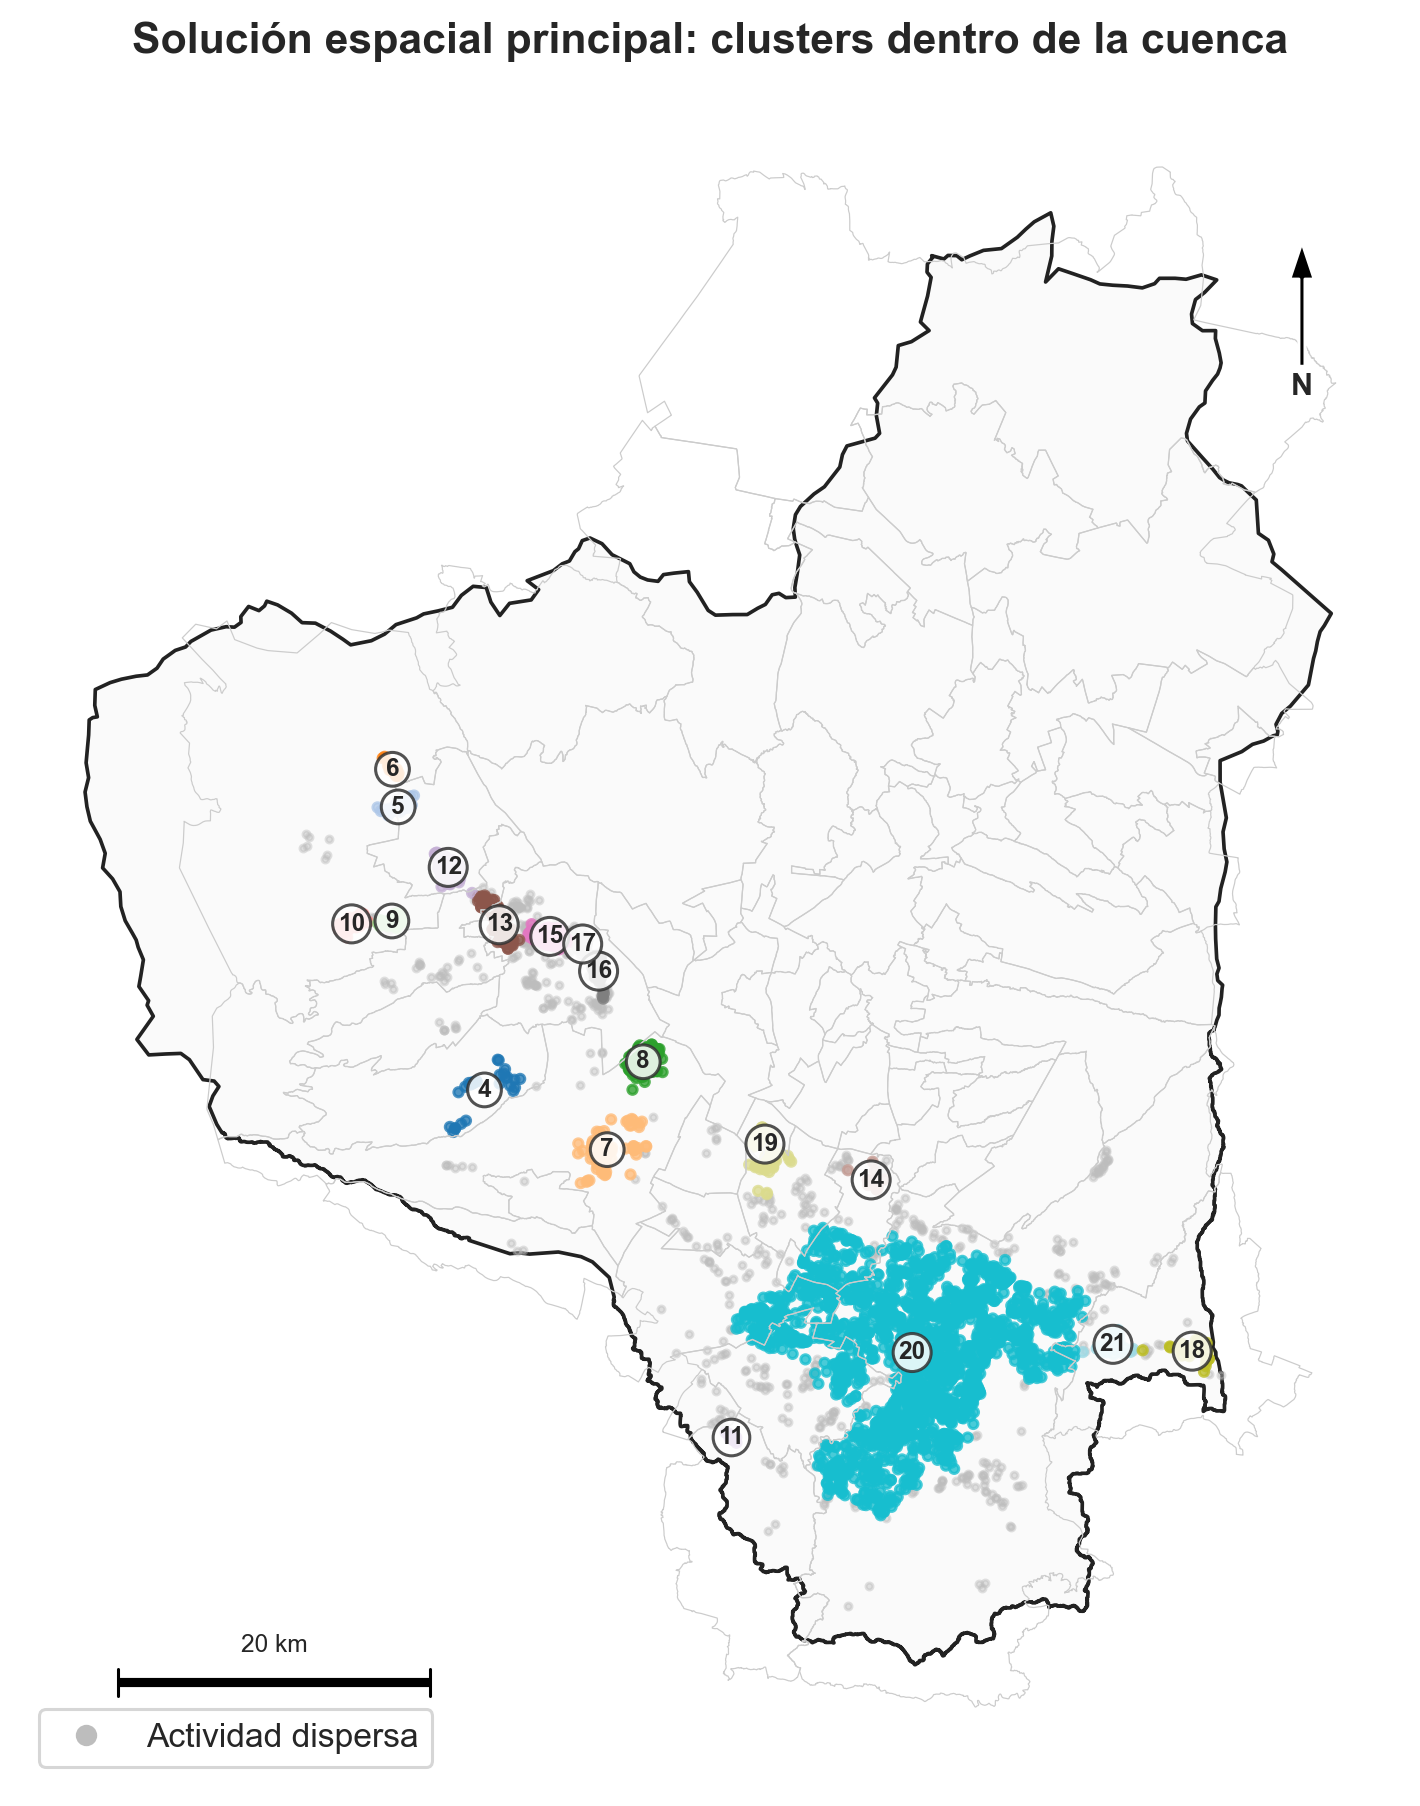
\includegraphics[width=.94\textwidth]{../../outputs/parte_2/13_figuras_finales/02_clusters_principales.png}
\caption{Concentraciones interiores de la solución seleccionada y actividad dispersa. Los colores representan membresía espacial, no contaminación.}
\end{figure}

\section{Principales concentraciones territoriales}

\subsection*{Santa Ana Xalmimilulco y Huejotzingo}

Santa Ana Xalmimilulco corresponde al cluster 8 y reúne 337 establecimientos. Es una concentración manufacturera compacta: 85.8\% tiene señal de confección, 55.8\% de maquila y 40.7\% de mezclilla o pantalón. La evidencia sugiere una organización productiva especializada que amerita verificar si operaciones de lavado, limpieza o acabado ocurren dentro de talleres registrados principalmente como confección. No debe suponerse que todas las unidades pertenecen al universo hídrico estricto.

La cabecera de Huejotzingo y localidades próximas forman el cluster 7, con 99 establecimientos dentro de la cuenca. Su perfil es más mixto y 44.4\% pertenece a lavandería/tintorería sectorial. Xalmimilulco y Huejotzingo deben tratarse como preguntas de campo distintas: el primero por cadenas de confección--maquila--mezclilla; el segundo por coexistencia de manufactura y servicios potencialmente húmedos.

\subsection*{Tlahuapan}

San Miguel Tianguistenco (cluster 9, 30 establecimientos) y San Rafael Ixtapalucan (cluster 10, 142) sobresalen por tejido e hilado: 80.0\% y 95.1\%, respectivamente. Santiago Coltzingo (cluster 6, 20) concentra señal de maquila en 16 unidades. Los porcentajes son altos, pero los tamaños de Tianguistenco y Coltzingo son pequeños; son candidatos para inspección focal, no bases para dimensionar obra.

\subsection*{San Martín Texmelucan, Tlanalapan y Moyotzingo}

El sistema no aparece como una sola masa homogénea. San Rafael Tlanalapan forma el cluster 13 con 149 unidades y una presencia importante de confección y proceso seco explícito. San Martín Texmelucan participa en los clusters 15 y 17; el 15 reúne 92 unidades y casi la mitad corresponde a lavandería/tintorería sectorial. Santa María Moyotzingo forma el cluster 16 con 51 unidades. La segunda etapa debe revisar conexiones funcionales entre estos núcleos sin fusionarlos automáticamente.

\subsection*{San Miguel Xoxtla--Coronango y Amozoc}

El cluster 19 reúne 100 establecimientos y se centra en San Miguel Xoxtla; 76\% tiene señal de confección. Su relación con Coronango debe estudiarse mediante movilidad productiva, drenaje e infraestructura, no solo por cercanía. Amozoc presenta dos concentraciones: clusters 18 y 21, con 32 y 31 unidades, y participaciones sectoriales de lavandería/tintorería cercanas a 41\%. Son núcleos pequeños que ameritan corroborar procesos reales.

\subsection*{Sistema Puebla--Cholula--Cuautlancingo}

El cluster 20 contiene 1,997 establecimientos y articula seis municipios y 14 localidades. No es una sola zona industrial ni una futura zona de servicio. Es una estructura metropolitana continua, con máximos locales conectados por bandas de establecimientos. La exploración interna reconoce 18 subnúcleos descriptivos, pero deja 44.5\% de sus puntos sin rama local bajo esa especificación; por ello los subnúcleos sirven para planear recorridos, no para sustituir silenciosamente la membresía principal.

\begin{figure}[H]\centering
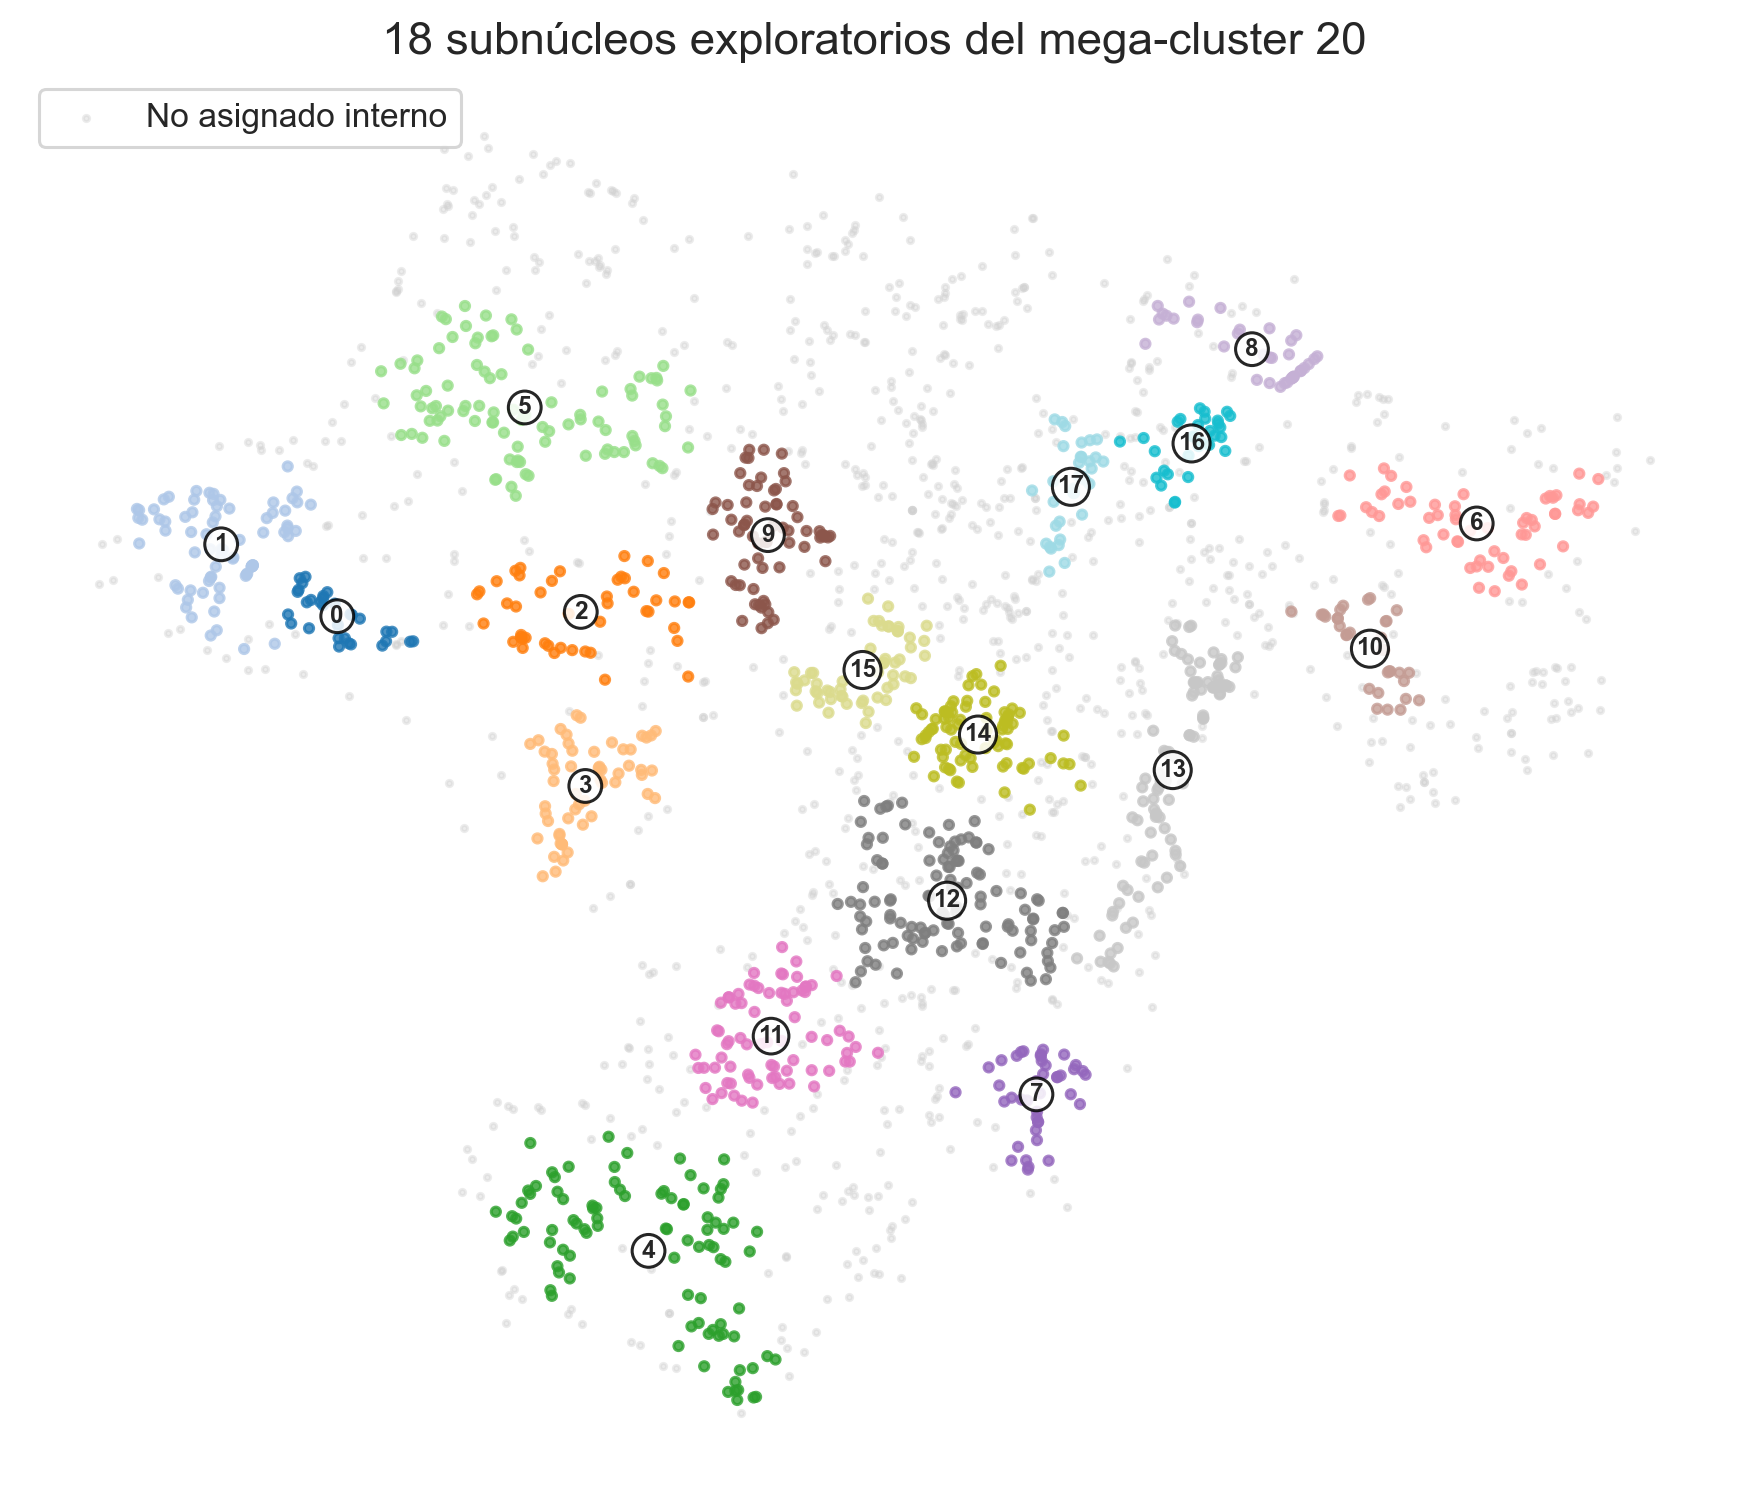
\includegraphics[width=.94\textwidth]{../../outputs/parte_2/14_segunda_pasada/figuras/03_subnucleos_mega_etiquetados.png}
\caption{Subnúcleos exploratorios del sistema metropolitano. Son estratos de lectura y validación, no nuevas zonas de servicio.}
\end{figure}

\section{Diferencias productivas entre clusters}

Las concentraciones no son intercambiables. El perfil posterior al clustering distingue núcleos manufactureros, territorios especializados en tejido/hilado, sistemas de confección--maquila--mezclilla y grupos mixtos con mayor presencia de lavandería/tintorería. Esta diferencia permite diseñar instrumentos de campo específicos: no conviene preguntar lo mismo a un taller de confección que a un establecimiento de acabado o a una lavandería registrada como servicio.

En Xalmimilulco, la mezcla de confección, maquila y mezclilla apunta a relaciones entre talleres y etapas productivas. En Tlahuapan, tejido/hilado domina las concentraciones de Ixtapalucan y Tianguistenco. Tlanalapan combina confección con procesos secos; Texmelucan y el cluster metropolitano presentan perfiles más mixtos. El ruido conserva numerosas microunidades manufactureras y no debe leerse como el opuesto económico de los clusters.

\begin{figure}[H]\centering
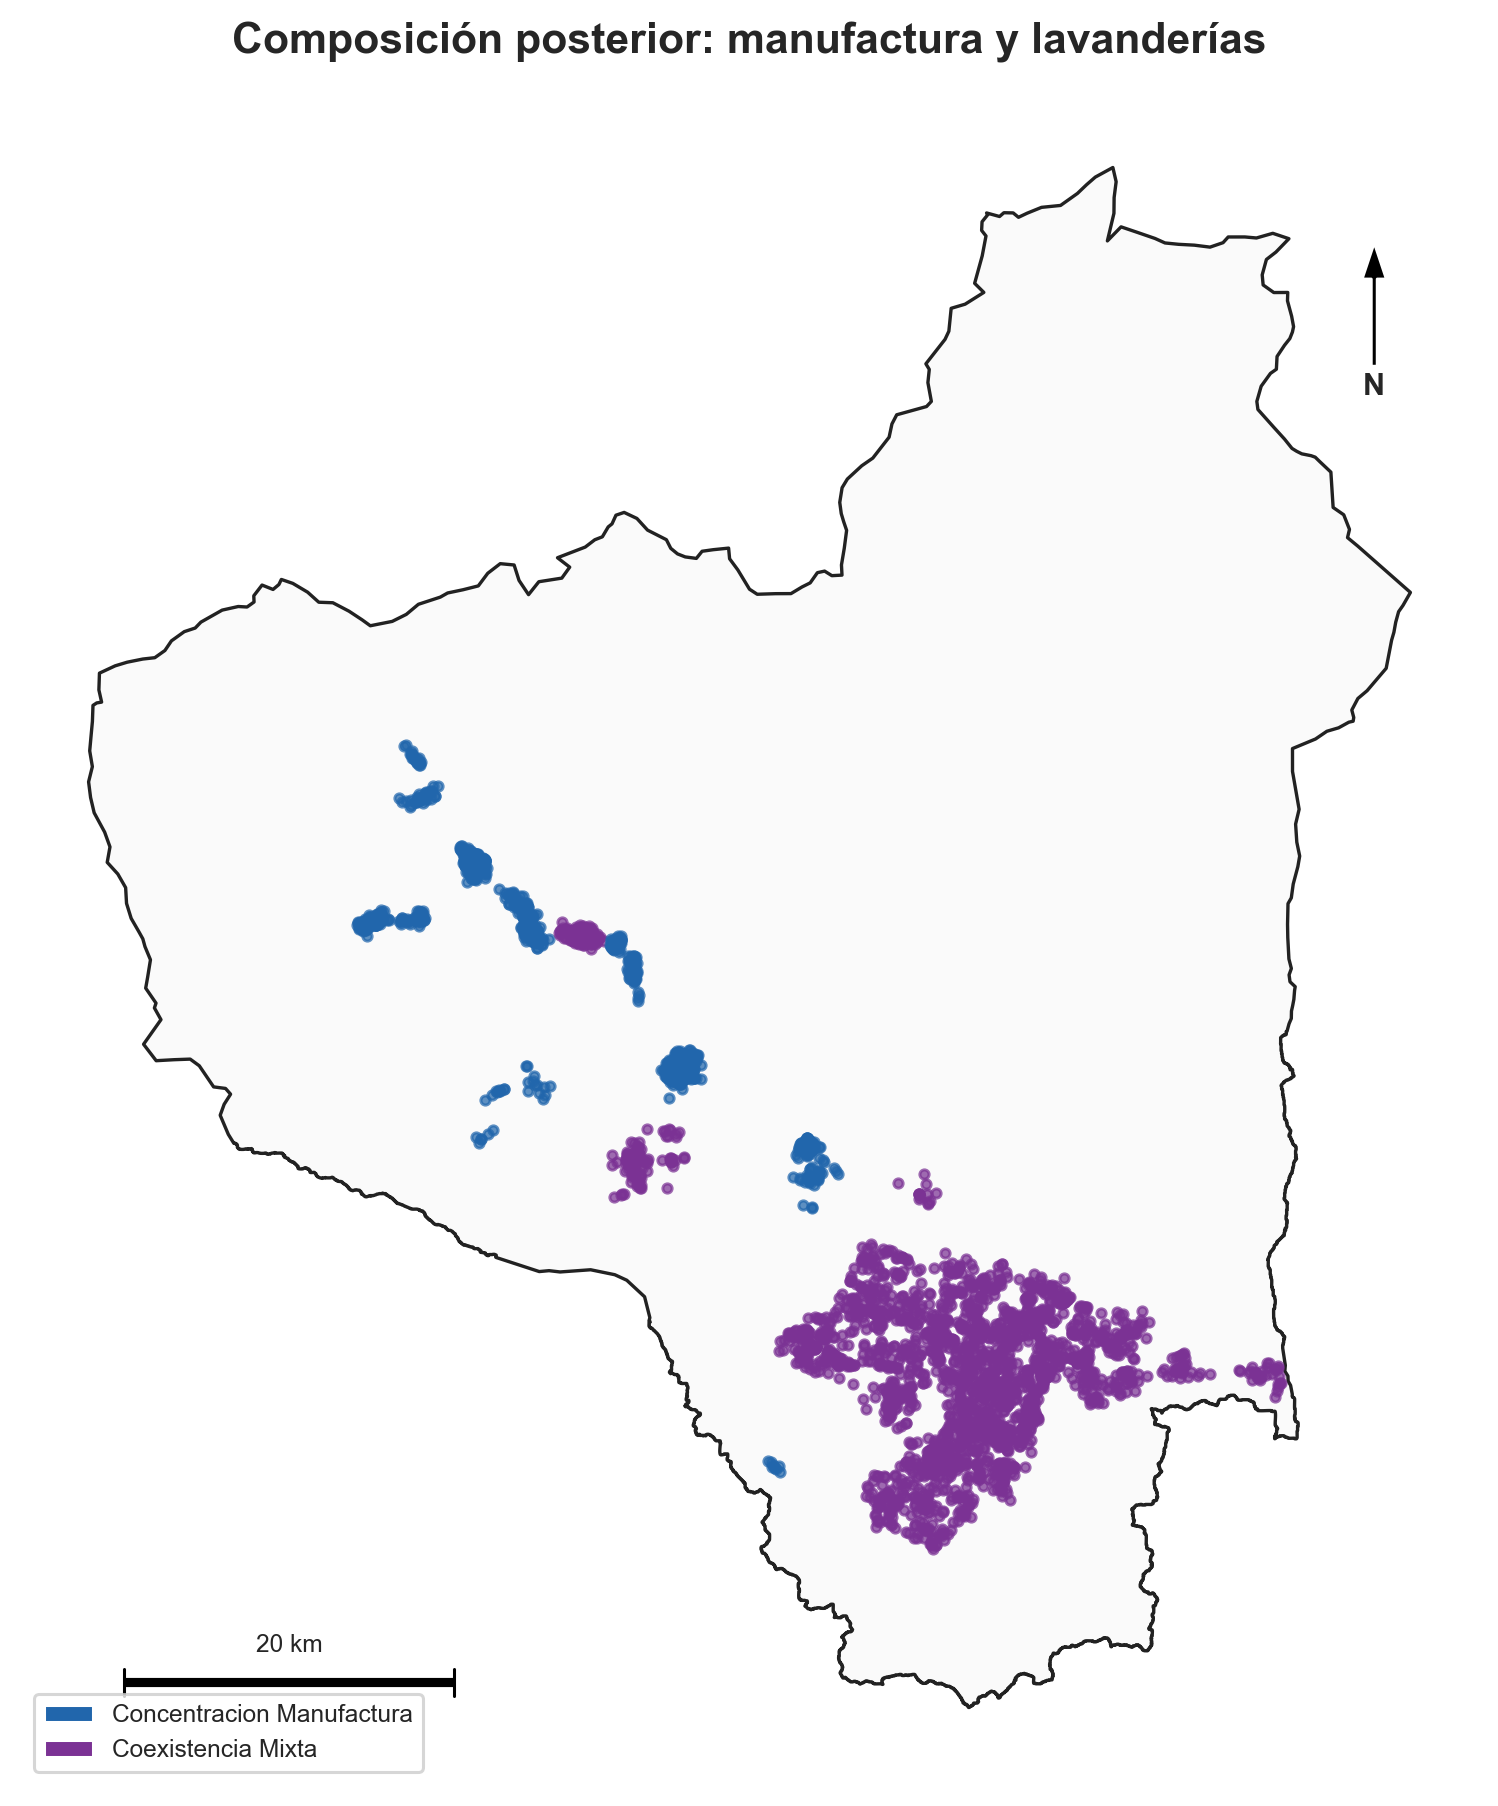
\includegraphics[width=.9\textwidth]{../../outputs/parte_2/13_figuras_finales/04_tipos_productivos_clusters.png}
\caption{Tipos productivos de las concentraciones, asignados después de fijar la geografía.}
\end{figure}

La sobrerrepresentación compara la frecuencia de una señal dentro de un cluster con su frecuencia regional. Por ejemplo, tejido/hilado aparece 10.62 veces más frecuentemente en el cluster 10 que en el universo interior; esto no significa 10.62 veces más producción. En el cluster 20, lavandería/tintorería sectorial abarca 1,185 unidades, pero solo 313 tienen señal húmeda explícita y 22 están etiquetadas como evidencia hídrica \texttt{SI}. Las categorías se traslapan y ninguna confirma por sí sola una lavandería industrial.

\begin{figure}[H]\centering
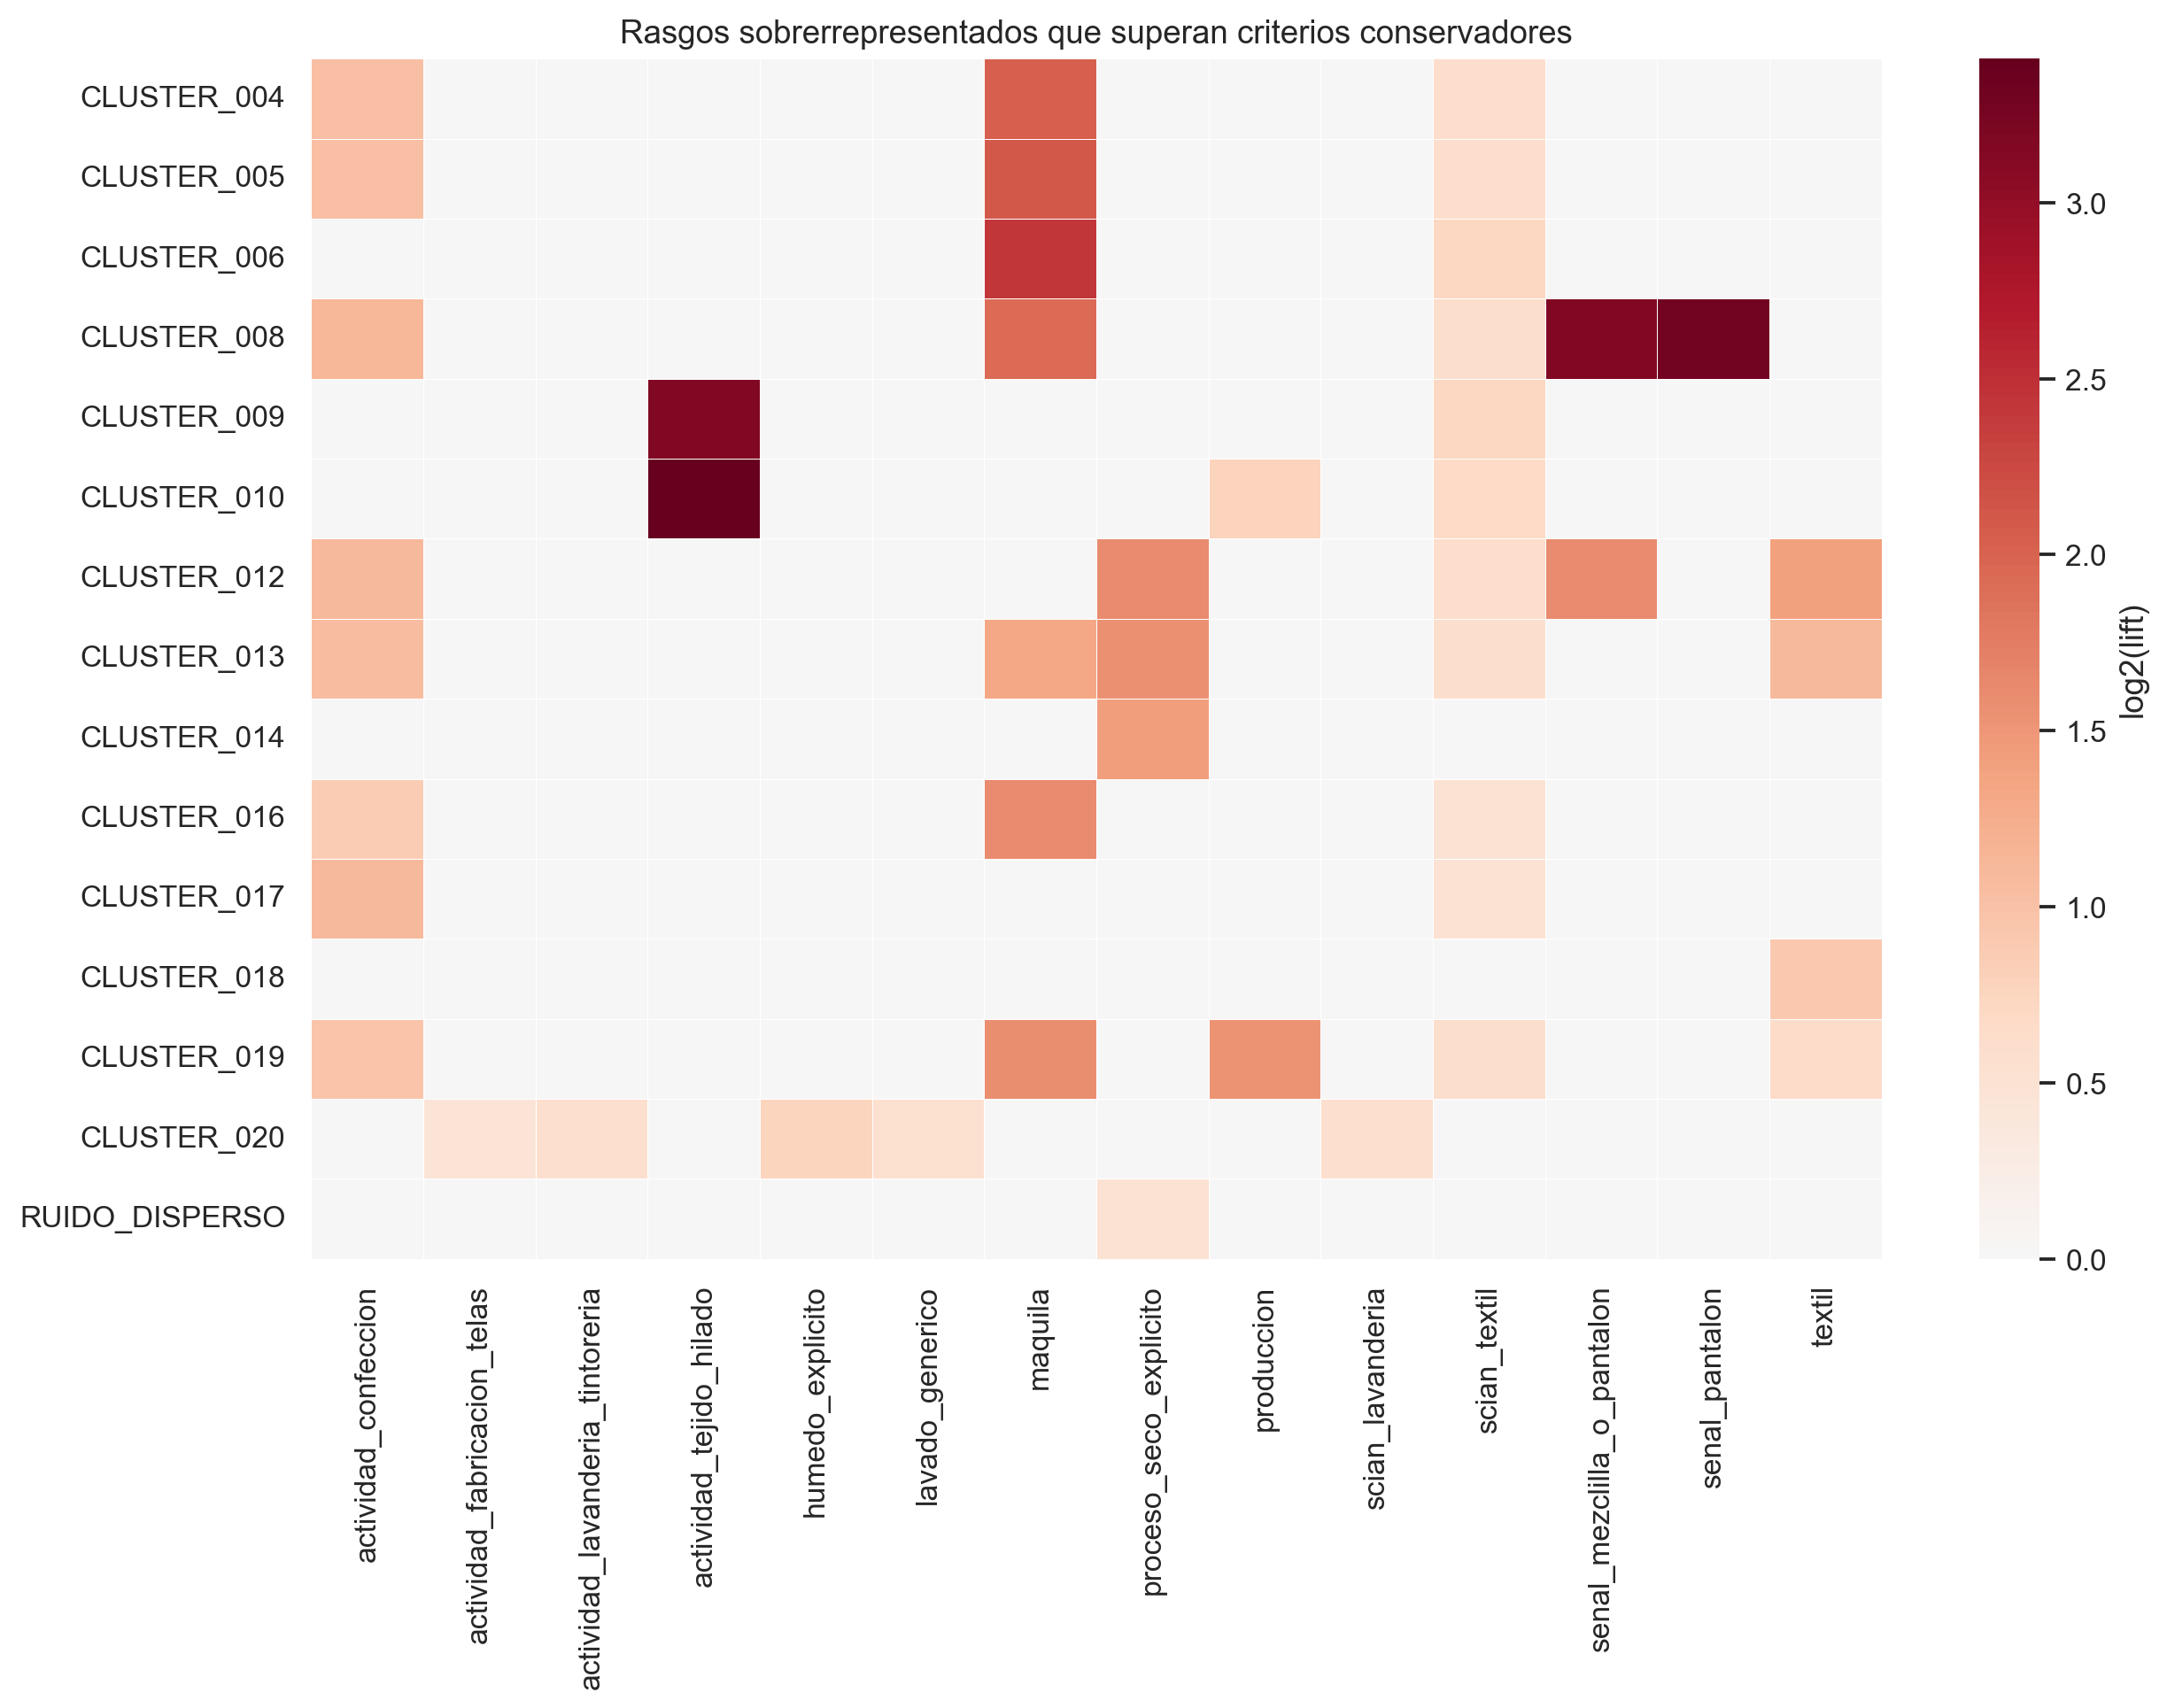
\includegraphics[width=.92\textwidth]{../../outputs/parte_2/13_figuras_finales/07_rasgos_distintivos.png}
\caption{Señales distintivas con suficiente tamaño y contraste dentro del universo observado.}
\end{figure}

\section{Robustez e incertidumbre}

La robustez se evaluó cambiando parámetros, comparando métodos y perturbando coordenadas 25 metros. La solución elegida obtiene el mayor puntaje, pero las alternativas HDBSCAN más cercanas producen particiones casi equivalentes. Este resultado es deseable: las concentraciones principales no dependen de un único ajuste, aunque la etiqueta exacta de algunos puntos sí cambia.

De los 4,365 establecimientos de detección, 4,107 son núcleos robustos, 94 tienen estabilidad intermedia y 164 son sensibles. Los cambios se concentran en bordes, corredores de baja densidad y transiciones entre cluster y ruido. Por eso cualquier directorio de visita debe incluir la persistencia de membresía y evitar tratar todos los puntos con la misma certeza.

\begin{figure}[H]\centering
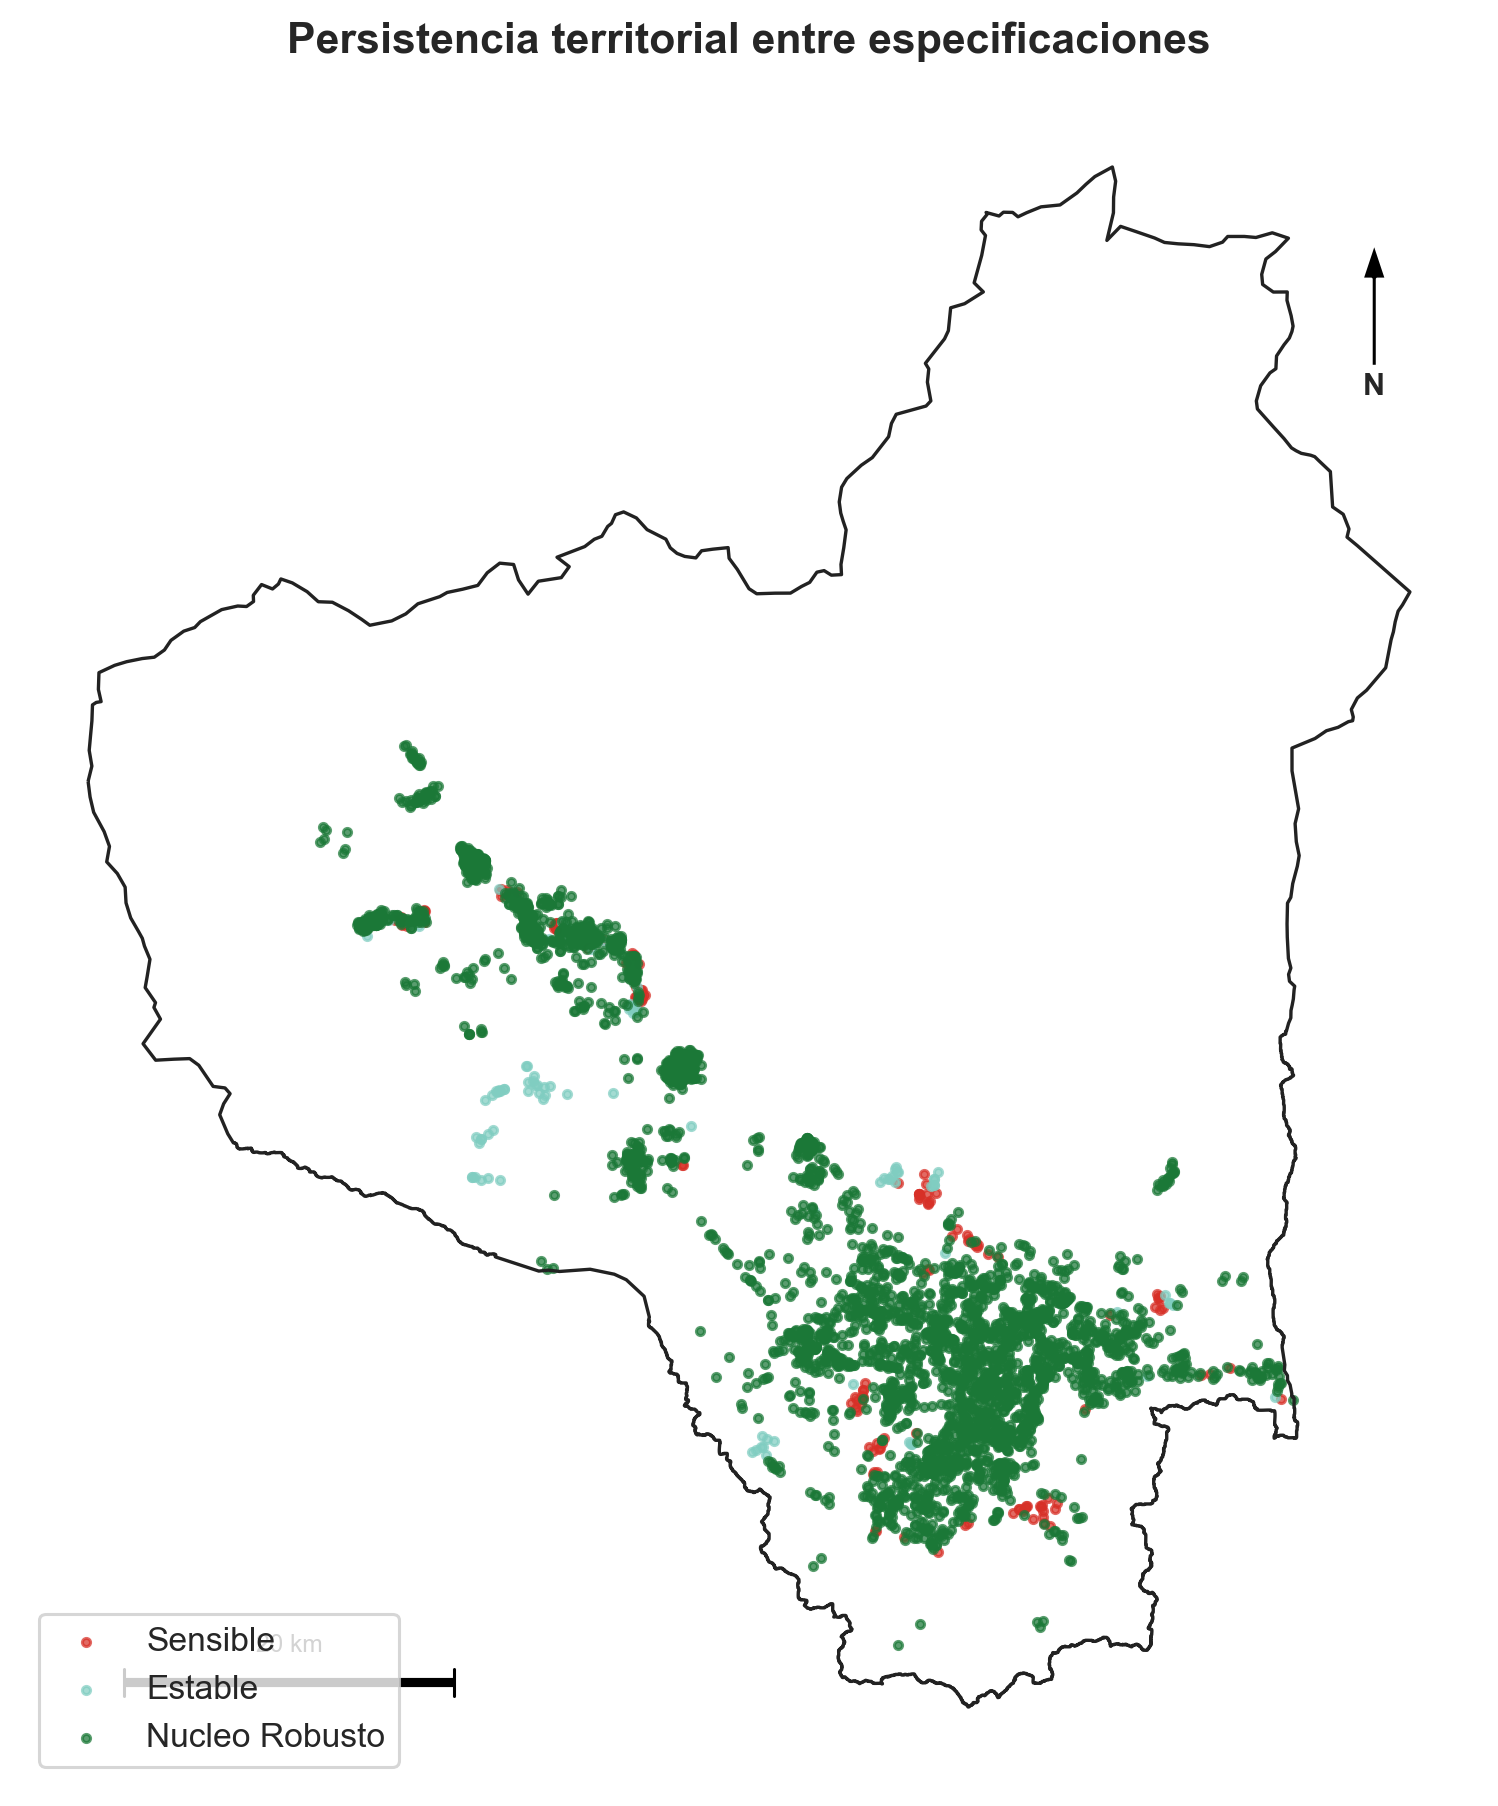
\includegraphics[width=.88\textwidth]{../../outputs/parte_2/13_figuras_finales/03_persistencia_territorial.png}
\caption{Persistencia territorial. Los puntos sensibles señalan dónde la delimitación requiere mayor cautela.}
\end{figure}

La incertidumbre tiene varias fuentes que el clustering no resuelve: vigencia y precisión de DENUE; nombres comerciales poco informativos; procesos no declarados; dependencia espacial entre establecimientos; límites de la red hidrográfica disponible; y ausencia de drenaje, caudal y calidad del agua. Las pruebas estadísticas del perfil se usan para ordenar asociaciones del universo observado; DENUE no es una muestra probabilística y esas pruebas no corrigen dependencia espacial.

\begin{figure}[H]\centering
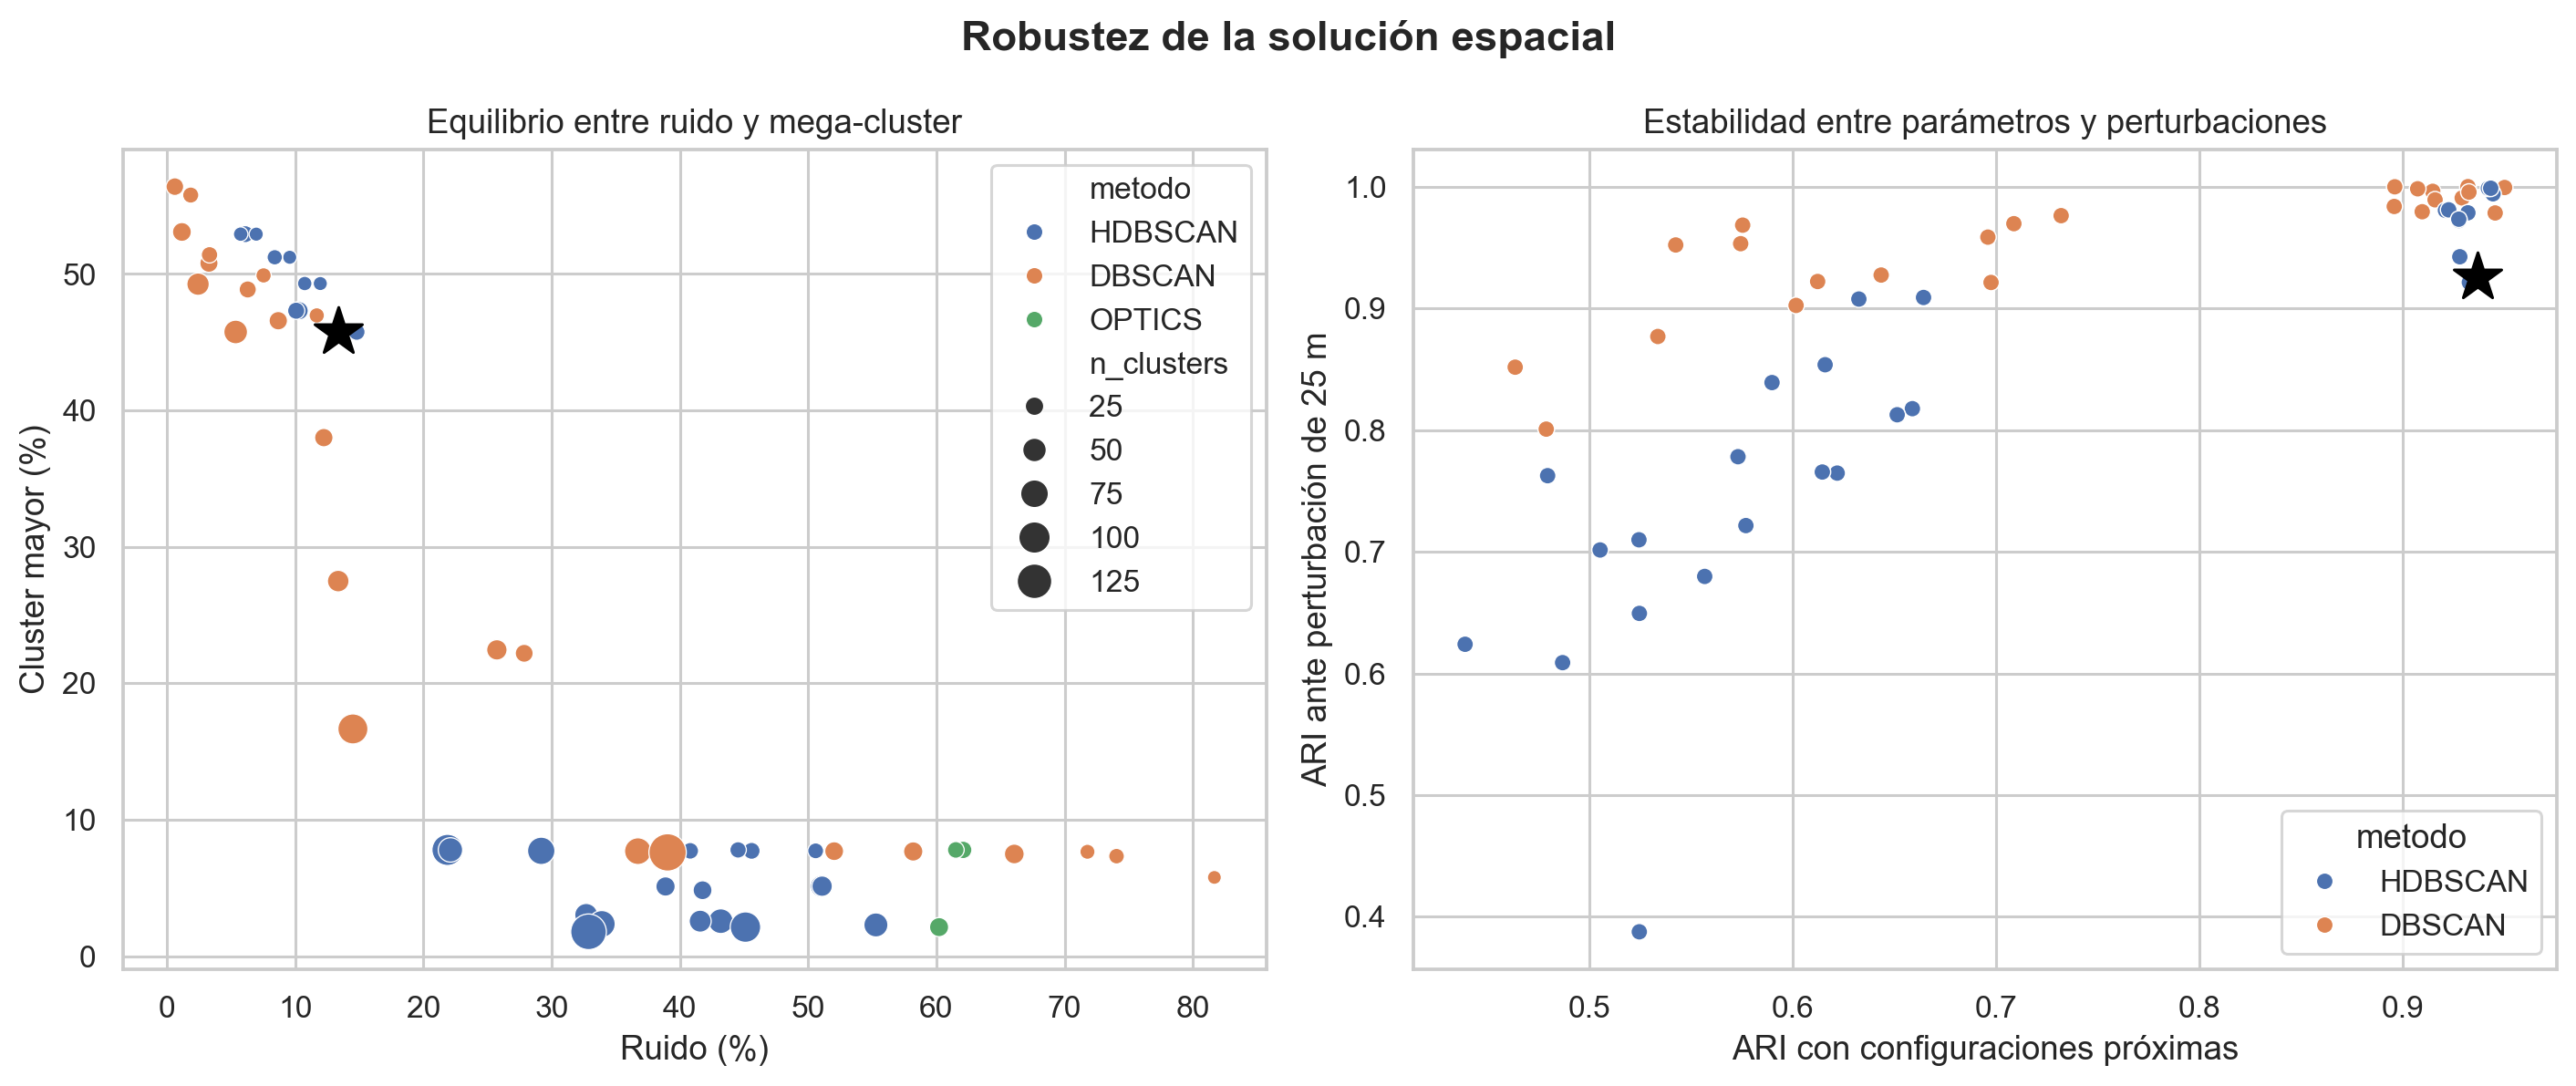
\includegraphics[width=.9\textwidth]{../../outputs/parte_2/13_figuras_finales/05_robustez_escenarios.png}
\caption{Equilibrio entre ruido, tamaño del grupo mayor y estabilidad de configuraciones seleccionadas.}
\end{figure}

\section{Zonas prioritarias para validación}

La prioridad debe entenderse como una secuencia de preguntas y no como un ranking automático de inversión.

\begin{tabularx}{\textwidth}{>{\bfseries}p{.28\textwidth}X}
\toprule
Territorio & Pregunta prioritaria de validación \\
\midrule
Santa Ana Xalmimilulco & Verificar vínculos entre confección, maquila, mezclilla y operaciones no registradas de lavado, limpieza o acabado. \\
Huejotzingo & Separar lavandería comercial, servicios a terceros y procesos textiles; identificar descargas y horarios reales. \\
Ixtapalucan, Tianguistenco y Coltzingo & Corroborar procesos asociados con tejido/hilado y maquila, consumo de agua y destino de residuos. \\
Texmelucan, Tlanalapan y Moyotzingo & Examinar conexiones productivas y sanitarias entre núcleos distintos; no asumir un solo corredor hidráulico. \\
Xoxtla--Coronango & Validar continuidad funcional, talleres activos y relación con redes de drenaje. \\
Amozoc & Distinguir lavanderías sectoriales de operaciones industriales y revisar la estabilidad de núcleos pequeños. \\
Puebla--Cholula--Cuautlancingo & Estratificar visitas por subnúcleo, actividad y persistencia; superponer red sanitaria y capacidad de tratamiento. \\
\bottomrule
\end{tabularx}

La selección de establecimientos para campo debe conservar ID DENUE, fuente, cluster, persistencia, señales productivas y modalidad amplia/estricta. Conviene incluir controles fuera de los núcleos y una fracción del ruido, porque validar únicamente los puntos más evidentes produciría una imagen sesgada de la actividad territorial.

\section{Qué no concluye el estudio}

\begin{itemize}
\item No identifica establecimientos contaminantes ni prueba incumplimiento.
\item No convierte una cercanía cartográfica a un río en ruta de descarga.
\item No demuestra que una categoría de lavandería/tintorería corresponda a lavandería industrial.
\item No estima consumo, caudal, carga contaminante, producción ni toxicidad.
\item No delimita áreas tributarias, cuencas sanitarias ni zonas de servicio.
\item No demuestra que el cluster metropolitano sea homogéneo o deba atenderse con una sola solución.
\item No convierte significancia estadística en causalidad, prioridad ambiental o viabilidad de obra.
\item No selecciona un trazo de colector, una planta o una inversión.
\end{itemize}

Los mapas son instrumentos de priorización. Una concentración puede aumentar la eficiencia de un recorrido o de un muestreo, pero la decisión hidráulica depende de pendientes, redes existentes, conexiones, puntos de descarga, caudales, tecnología de tratamiento, permisos y costos. Estos datos no están contenidos en DENUE.

\section{Siguientes pasos}

El siguiente avance debe integrar las concentraciones económicas identificadas con la \textbf{hidrología, el relieve y la red de drenaje}. El propósito es entender por qué rutas potenciales salen los residuos líquidos de estas agrupaciones, cómo se desplazan por gravedad o bombeo a través de la infraestructura sanitaria y de la superficie, en qué puntos pueden incorporarse a cauces o cuerpos de agua y hacia dónde continúan fluyendo. Esta reconstrucción debe combinarse con la información existente sobre colectores, atarjeas, pozos de visita, puntos de captación o intercepción, descargas conocidas y plantas de tratamiento, incluyendo su ubicación, área atendida, capacidad y estado operativo.

La integración permitirá pasar de una concentración de establecimientos a una hipótesis de funcionamiento hídrico territorial: qué agrupaciones podrían compartir una ruta de drenaje, qué receptores quedarían aguas abajo, qué infraestructura puede captar o tratar los flujos y dónde existen vacíos de información o posibles desconexiones. Las rutas resultantes serán hipótesis para verificar mediante inspección, aforo, trazadores, muestreo y datos del organismo operador; no se inferirán como descargas comprobadas únicamente por pendiente, cercanía o coincidencia cartográfica. Se propone esta secuencia:

\begin{enumerate}
\item Integrar establecimientos y clusters con cauces, cuerpos de agua, subcuencas, modelo de elevación y pendientes; después incorporar atarjeas, colectores, pozos de visita, cárcamos, captadores o interceptores, puntos de descarga y plantas de tratamiento existentes.
\item Diseñar una validación estratificada por territorio, perfil productivo, evidencia hídrica y persistencia, incluyendo unidades dispersas como contraste.
\item Verificar actividad, proceso, materias primas, limpieza de equipo, punto de descarga, horario, pretratamiento y estado operativo.
\item Realizar aforos y muestreo fisicoquímico con cadena de custodia en establecimientos, drenajes y receptores seleccionados.
\item Delimitar áreas realmente tributarias y rutas posibles por gravedad o bombeo; separar proximidad euclidiana de conexión hidráulica.
\item Evaluar capacidad disponible, tecnología y compatibilidad de efluentes de las plantas existentes.
\item Construir escenarios de caudal y carga con incertidumbre y comparar alternativas de prevención, pretratamiento, conducción y tratamiento mediante CAPEX, OPEX, riesgo, beneficio ambiental, permisos y gobernanza.
\end{enumerate}

\idea{Lo ganado con este proyecto es una reducción auditable del territorio: de miles de registros aislados a concentraciones, perfiles y preguntas verificables. La próxima decisión no es dónde construir, sino dónde y cómo producir la evidencia hidráulica y ambiental que todavía falta.}

\subsection*{Acceso a resultados}

La matriz maestra está en \path{outputs/parte_2/01_matriz/}; la solución espacial en \path{outputs/parte_2/06_clusters/}; los perfiles en \path{outputs/parte_2/07_perfiles/}; los contrastes en \path{outputs/parte_2/08_sobrerrepresentacion/}; el atlas en \path{outputs/parte_2/12_atlas/}; y los subnúcleos y el explorador interactivo en \path{outputs/parte_2/14_segunda_pasada/}. El reporte maestro documenta métodos, advertencias y trazabilidad completa.

\appendix
\section{Diccionario de palabras y conceptos clave}

Este diccionario fija el sentido de los términos utilizados en el reporte. Las definiciones son operativas para este proyecto y deben leerse junto con los límites metodológicos señalados en el texto.

\footnotesize
\begin{longtable}{>{\bfseries\raggedright\arraybackslash}p{.25\textwidth}>{\raggedright\arraybackslash}p{.68\textwidth}}
\toprule
Término & Definición y uso en el reporte \\
\midrule
\endfirsthead
\toprule
Término & Definición y uso en el reporte \\
\midrule
\endhead
Área tributaria & Superficie cuyos flujos llegan efectivamente a un punto de drenaje o tratamiento. Debe delimitarse con topografía e infraestructura; no coincide necesariamente con un cluster. \\
Atarjea & Conducto local de la red sanitaria que recibe descargas y las conduce hacia colectores de mayor jerarquía. \\
Captador o interceptor & Infraestructura que recibe, desvía o intercepta un flujo antes de su llegada a otro conducto o cuerpo receptor. Su existencia y funcionamiento deben verificarse con el operador. \\
Cauce & Conducto natural o artificial por el que fluye agua. La cercanía de un establecimiento a un cauce no demuestra que descargue en él. \\
Cluster & Agrupamiento de establecimientos próximos bajo una configuración del algoritmo. Es una unidad analítica, no una fuente comprobada de contaminación ni una zona de servicio. \\
Colector & Conducto principal que reúne aguas de ramales o atarjeas. Para proponer conexiones se necesitan trazo, cota, diámetro, capacidad y estado operativo. \\
Concentración espacial & Acumulación de establecimientos más próximos entre sí que bajo el patrón circundante. Describe geografía económica; no demuestra contaminación. \\
Cuenca del Alto Atoyac & Polígono hidrológico adoptado como área principal de interpretación. El análisis conservó contexto exterior para controlar el efecto de borde. \\
Cuerpo de agua & Río, arroyo, canal, presa u otro receptor superficial. Su relación con residuos requiere demostrar una ruta hidráulica. \\
DENUE & Directorio Estadístico Nacional de Unidades Económicas del INEGI. Aporta identificación, actividad declarada y coordenadas; no documenta por sí solo procesos, consumos o descargas. \\
Descarga & Salida efectiva de agua residual desde un establecimiento o infraestructura. Debe verificarse mediante inspección, registro o medición; no se deduce por proximidad. \\
Drenaje & Red de conductos, conexiones, pozos, cárcamos y estructuras que transportan aguas residuales o pluviales. Su funcionamiento real puede diferir del trazo cartográfico. \\
Efecto de borde & Distorsión causada al cortar vecinos en el límite de la cuenca. Se redujo detectando clusters con puntos municipales interiores y exteriores próximos. \\
Evidencia hídrica & Etiqueta construida a partir de reglas textuales o fuente MH para priorizar revisión. Sus estados \texttt{SI} y \texttt{REVISAR} no equivalen a descarga confirmada. \\
Fuente MH & Evidencia independiente derivada del trabajo de campo de Mary Helen Figueroa y Mayra Jaqueline Ramírez, enlazada con IDs DENUE cuando fue posible. \\
HDBSCAN & Método de clustering por densidad capaz de representar agrupamientos con densidades variables y asignar probabilidades de pertenencia. \\
Húmedo explícito & Señal textual que menciona operaciones potencialmente relacionadas con agua. Es evidencia registral, no verificación del proceso actual. \\
Lavado genérico contextualizado & Mención de lavado interpretada junto con vocabulario textil u otras señales para reducir ambigüedad. \\
Lavandería/tintorería sectorial & Clasificación basada en SCIAN o actividad registrada. Incluye posibles servicios comerciales y no equivale a lavandería industrial verificada. \\
Lift & Razón entre la prevalencia de una señal en un cluster y su prevalencia en los 4,010 establecimientos interiores. Valores mayores que uno indican sobrerrepresentación descriptiva. \\
Mega-cluster & Nombre descriptivo del cluster 20, con 1,997 establecimientos y continuidad metropolitana. No implica homogeneidad ni una solución hidráulica única. \\
Membresía & Asignación de un establecimiento a un cluster o al ruido bajo la configuración seleccionada. \\
MH & Abreviatura utilizada para la fuente de trabajo de campo descrita anteriormente; se conserva separada de DENUE. \\
Planta de tratamiento & Instalación que recibe y trata aguas residuales. Para evaluar su utilidad se requieren capacidad real, tecnología, cargas admisibles, cobertura y estado operativo. \\
Prevalencia & Proporción de establecimientos de un conjunto que presenta una señal determinada. No mide producción, caudal ni carga. \\
Priorización territorial & Selección de zonas y preguntas para producir evidencia adicional. No constituye una recomendación automática de colector o inversión. \\
Proceso seco explícito & Señal textual asociada con operaciones que no declaran uso de agua. No descarta limpieza húmeda u operaciones no registradas. \\
Relieve & Forma y elevación del terreno. Permite estudiar pendientes y rutas gravitacionales, pero debe combinarse con la red construida y verificarse en campo. \\
Residuo líquido o agua residual & Flujo resultante de una operación o uso del agua. Su volumen, composición y destino no se estiman a partir del número de establecimientos. \\
Ruido o actividad dispersa & Establecimientos no asignados a un cluster bajo la configuración seleccionada. No significa error, irrelevancia ni ausencia de impacto ambiental. \\
SCIAN & Sistema de Clasificación Industrial de América del Norte. Organiza actividades económicas declaradas y sirve para construir el universo y los perfiles. \\
Señal productiva & Indicador derivado de SCIAN o texto comercial, como confección, maquila, mezclilla o tejido/hilado. Describe hipótesis de actividad. \\
Subnúcleo & Partición exploratoria interna del mega-cluster utilizada para organizar recorridos. No reemplaza la membresía principal ni define áreas tributarias. \\
Universo sectorial & Conjunto amplio de actividades textiles, confección y lavandería/tintorería usado como denominador principal del análisis regional. \\
Universo estricto & Modalidad que exige evidencia más directa y excluye lavanderías sin señal adicional. Se usa como contraste de sensibilidad, no como verdad definitiva. \\
Validación de campo & Comprobación directa de actividad, proceso, uso de agua, descarga, conexión e infraestructura mediante visita y evidencia documentada. \\
\bottomrule
\end{longtable}
\normalsize

\end{document}
